\documentclass{standalone}
\usepackage{graphicx}	
\usepackage{amssymb, amsmath}
\usepackage{color}
\usepackage{wasysym}

\usepackage{tikz}
\usetikzlibrary{intersections, backgrounds}
\usepackage{pgfmath}

\definecolor{light}{RGB}{220, 188, 188}
\definecolor{mid}{RGB}{185, 124, 124}
\definecolor{dark}{RGB}{143, 39, 39}
\definecolor{highlight}{RGB}{180, 31, 180}
\definecolor{gray10}{gray}{0.1}
\definecolor{gray20}{gray}{0.2}
\definecolor{gray30}{gray}{0.3}
\definecolor{gray40}{gray}{0.4}
\definecolor{gray60}{gray}{0.6}
\definecolor{gray70}{gray}{0.7}
\definecolor{gray80}{gray}{0.8}
\definecolor{gray90}{gray}{0.9}
\definecolor{gray95}{gray}{0.95}

\newcommand*{\offset}{0.025}

\begin{document}

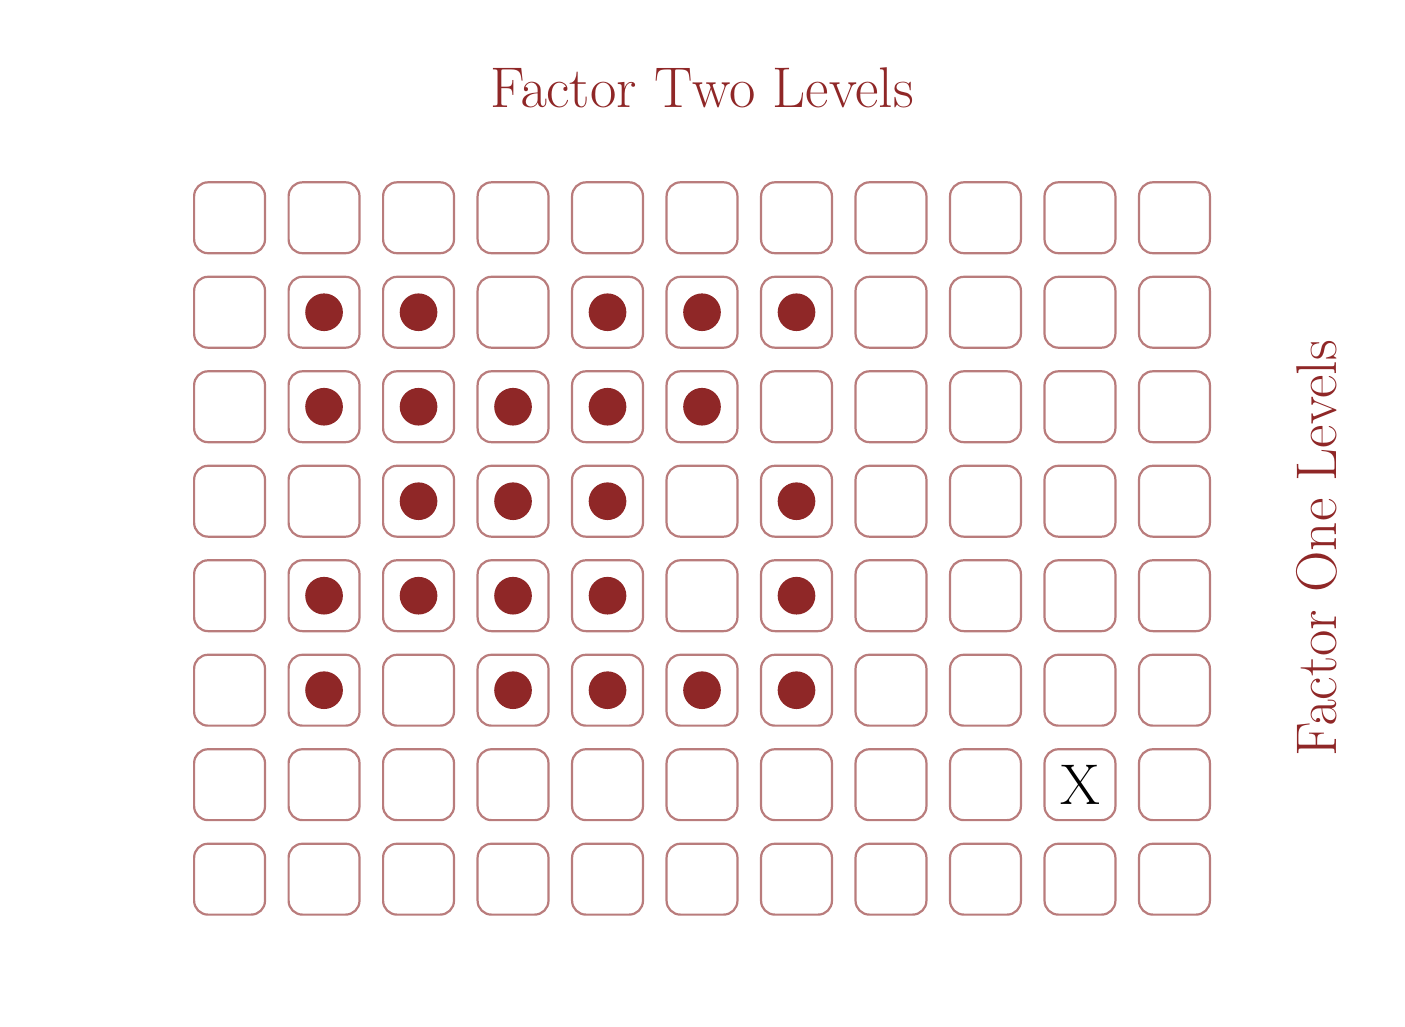
\begin{tikzpicture}[scale=0.3, thick]

\pgfmathsetmacro{\cx}{2}
\pgfmathsetmacro{\cy}{3}

\draw[white] (-28.5, -19) rectangle (28.5, 22);

\node[dark, rotate=90] at (26, 0) { \huge Factor One Levels };
\node[dark] at (0, 19.5) { \huge Factor Two Levels };

\foreach \x in {-20, -16, ..., 20} {
  \foreach \y in {-14, -10, ..., 14} {
    \draw[mid, rounded corners=5] (-1.5 + \x, -1.5 + \y) rectangle +(3, 3);
  }
}

\filldraw[draw=dark, fill=dark] (-16, 10) circle (0.75);
\filldraw[draw=dark, fill=dark] (-16, 6) circle (0.75);
\filldraw[draw=dark, fill=dark] (-16, -2) circle (0.75);
\filldraw[draw=dark, fill=dark] (-16, -6) circle (0.75);

\filldraw[draw=dark, fill=dark] (-12, 10) circle (0.75);
\filldraw[draw=dark, fill=dark] (-12, 6) circle (0.75);
\filldraw[draw=dark, fill=dark] (-12, 2) circle (0.75);
\filldraw[draw=dark, fill=dark] (-12, -2) circle (0.75);

\filldraw[draw=dark, fill=dark] (-8, 6) circle (0.75);
\filldraw[draw=dark, fill=dark] (-8, 2) circle (0.75);
\filldraw[draw=dark, fill=dark] (-8, -2) circle (0.75);
\filldraw[draw=dark, fill=dark] (-8, -6) circle (0.75);

\filldraw[draw=dark, fill=dark] (-4, 10) circle (0.75);
\filldraw[draw=dark, fill=dark] (-4, 6) circle (0.75);
\filldraw[draw=dark, fill=dark] (-4, 2) circle (0.75);
\filldraw[draw=dark, fill=dark] (-4, -2) circle (0.75);
\filldraw[draw=dark, fill=dark] (-4, -6) circle (0.75);

\filldraw[draw=dark, fill=dark] (0, 10) circle (0.75);
\filldraw[draw=dark, fill=dark] (0, 6) circle (0.75);
\filldraw[draw=dark, fill=dark] (0, -6) circle (0.75);

\filldraw[draw=dark, fill=dark] (4, 10) circle (0.75);
\filldraw[draw=dark, fill=dark] (4, 2) circle (0.75);
\filldraw[draw=dark, fill=dark] (4, -2) circle (0.75);
\filldraw[draw=dark, fill=dark] (4, -6) circle (0.75);

\node at (16, -10) { \huge X };


\end{tikzpicture}

\end{document}  